\section{Systematic uncertainties}
\label{sec:systematics1}
The sources of systematic uncertainties are summarized as
follows:
\begin{itemize}
\item Background-related systematic uncertainties: background shape parametrization.
\item Signal-related systematics uncertainties: the determination of W/Z-tagging efficiency, jet energy scale(JES), jet energy resolution(JER), luminosity, PDF, and pile up.
\end{itemize}

\subsection{Background shape parametrization}
\label{sec:background1}

We model the shape of the QCD background in the dijet spectrum 
using a simple parametrization which has been successfully deployed in
previous searches in the dijet mass spectrum~\cite{cmsdijet}.
Note in the limit setting, we employ a background plus signal fit. Here
we show the background only fit to prove that data is dominated by background. 
The background model is given in Equation~(\ref{eqParam1}):
\begin{equation}
\frac{{\rm d}N}{{\rm d}m} = 
\frac{P_{0} (1 - m/\sqrt{s})^{P_{1}}}{(m/\sqrt{s})^{P_{2}
}} .
\label{eqParam1}
\end{equation}
\noindent where $m$ denotes the dijet mass and $\sqrt{s}$  is the center of collision energy for pp process.
$P_0$ acts as a normalization parameter for the probability
density function, and $P_1$, $P_2$ describe its shape.
It has been checked by a Fisher F-test that no additional parameter is needed to describe the distributions.

Figure~\ref{fig:BG} show the dijet mass spectra for
single and double $\PW/\cPZ$-tagged data, fitted to Equation~(\ref{eqParam1}) and the bottom panes show corresponding pull
distributions, demonstrating the agreement between the background-only
probability density function and the data.

No sizable deviation from the background-only hypothesis is seen,
exclusion limits are set on the product of cross section, acceptance, and branching fraction for
the five considered final states: qW, qZ, WW, WZ, and ZZ.


\begin{figure}[th!b]
\centering
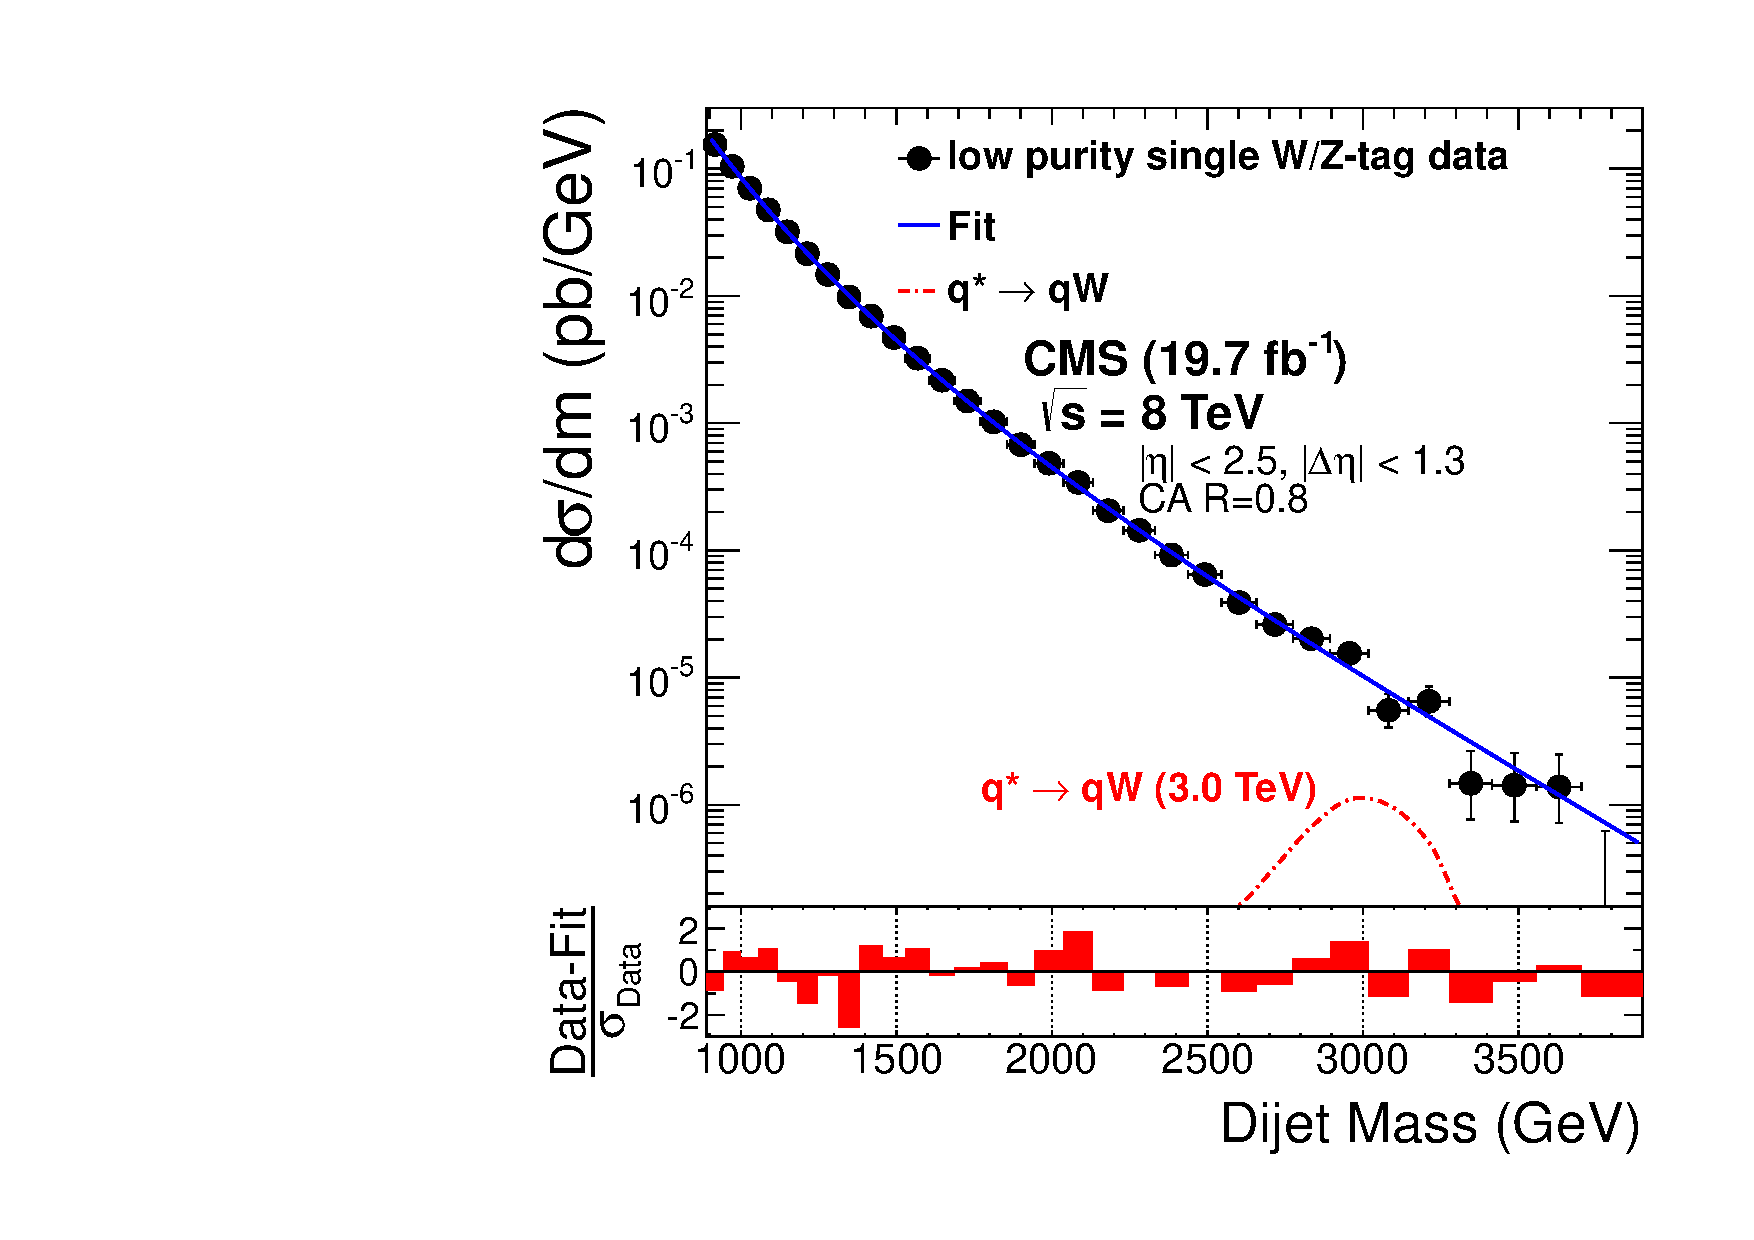
\includegraphics[width=0.49\textwidth]{EXO-12-024/figs/MediumPuriqVFitAndPull.pdf}
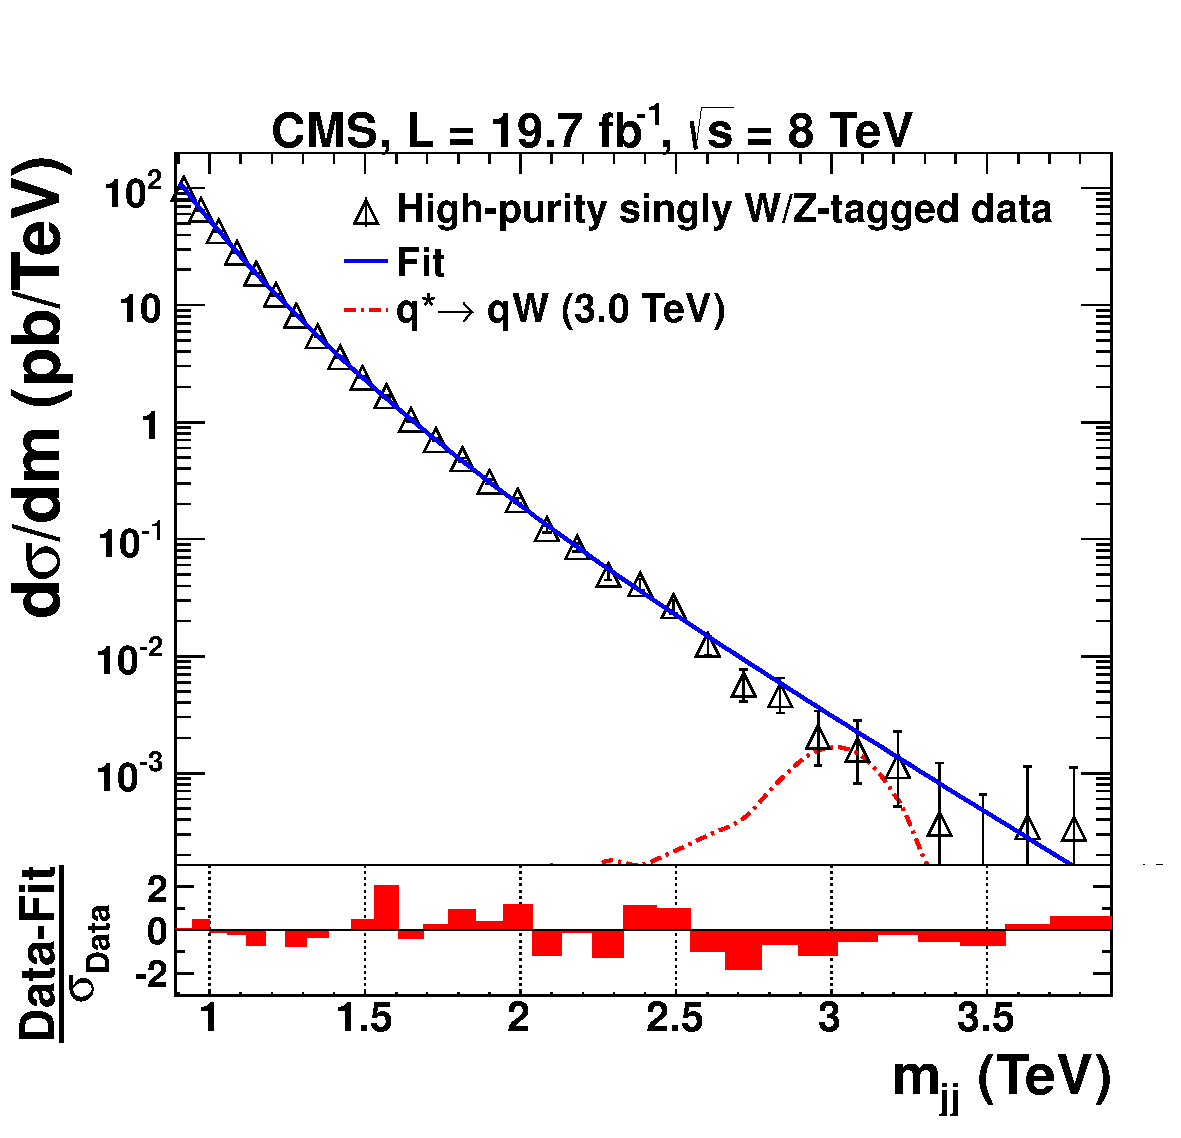
\includegraphics[width=0.49\textwidth]{EXO-12-024/figs/HighPuriqVFitAndPull.pdf}
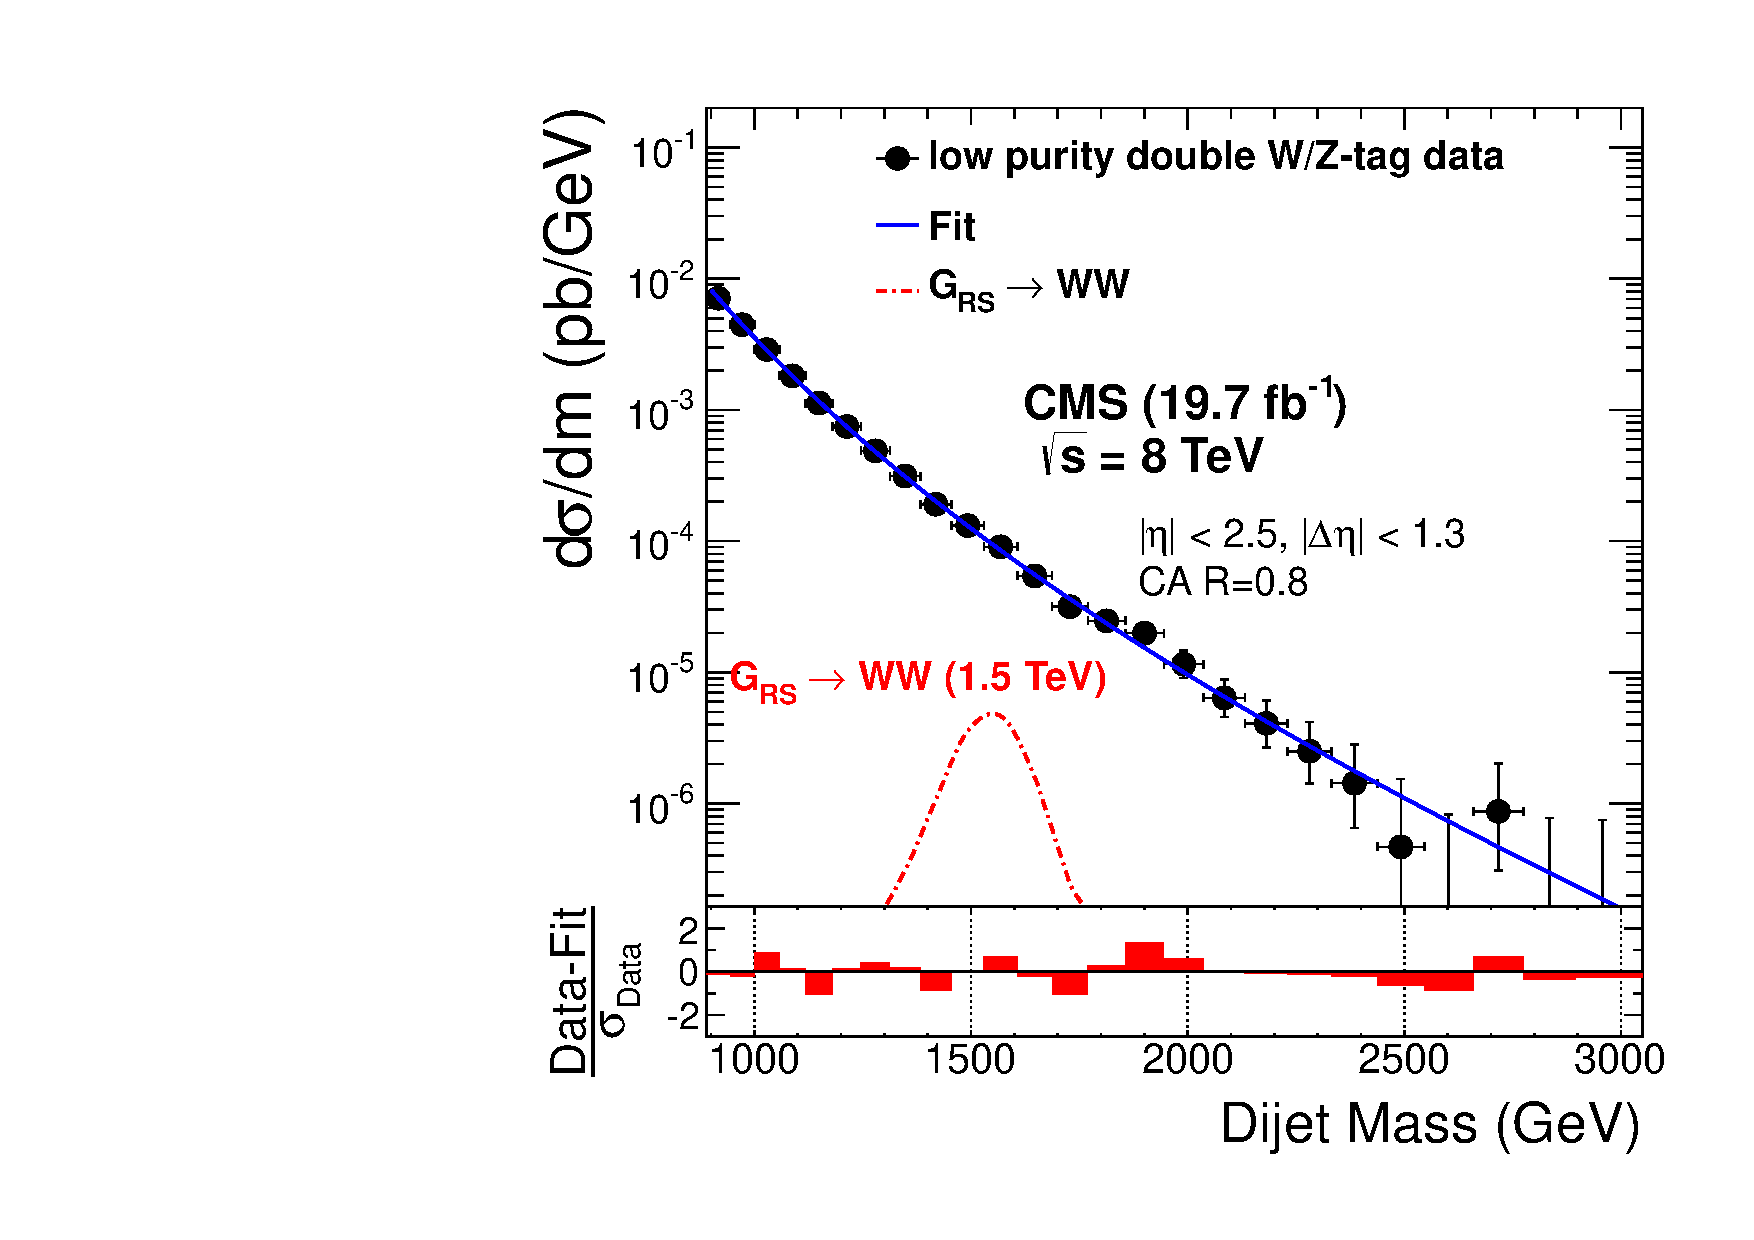
\includegraphics[width=0.49\textwidth]{EXO-12-024/figs/MediumPuriVVFitAndPull.pdf}
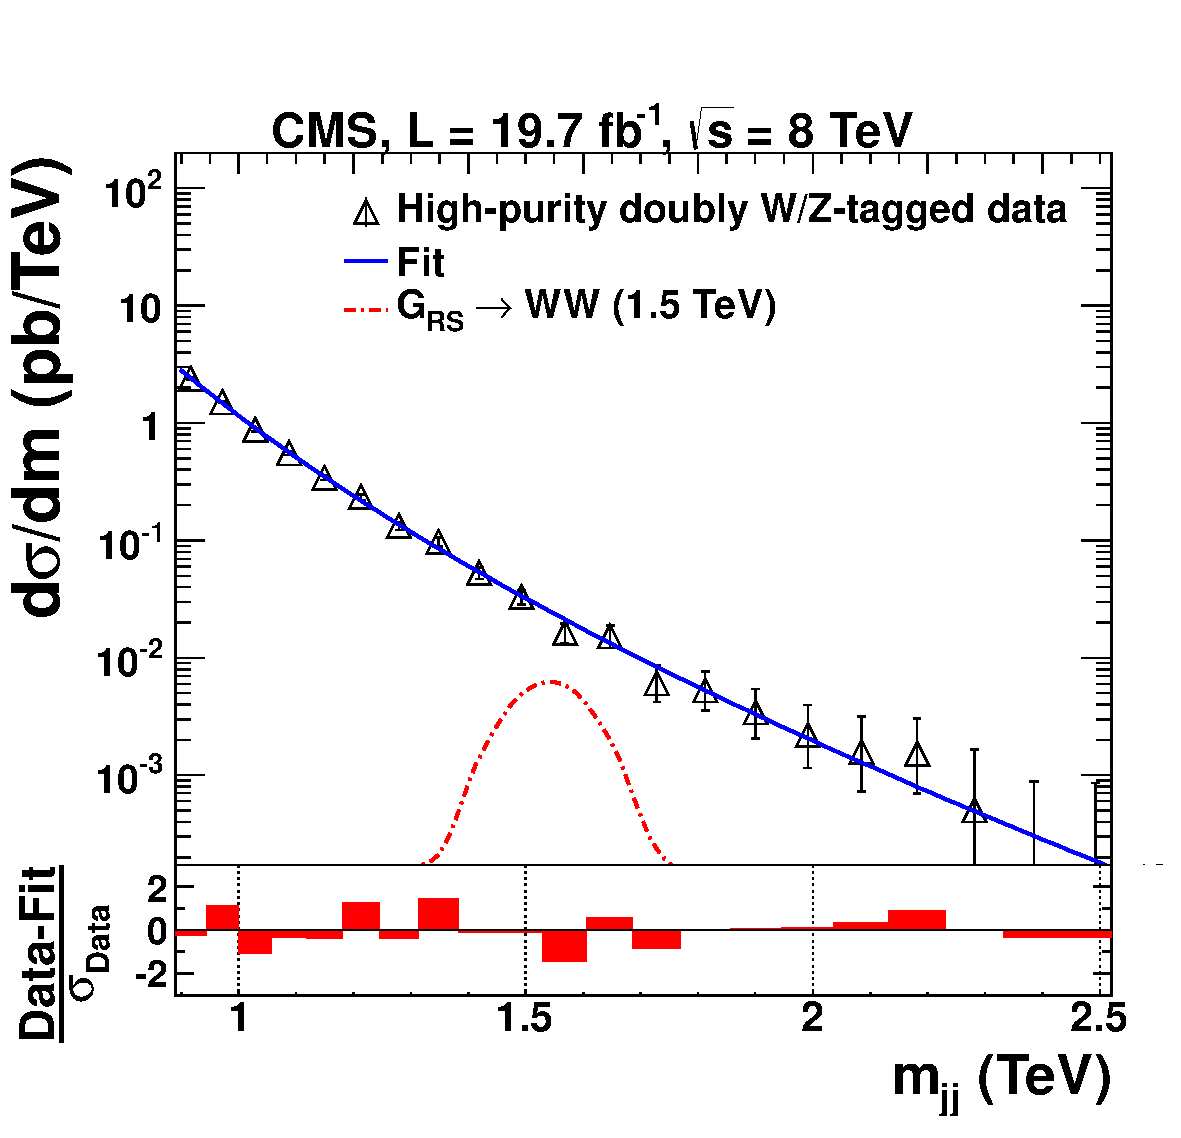
\includegraphics[width=0.49\textwidth]{EXO-12-024/figs/HighPuriVVFitAndPull.pdf}
 \caption{
   Distribution in ${\rm m_{jj} }$, respectively, for
   (upper left) singly-tagged LP events and (upper right) HP events, and for (lower left) doubly-tagged
   LP events and (lower right) HP events. The solid curves represent the
   results of fitting Eq.~(\ref{eqParam}) to the data. The
   distribution for $q^*\to q \PW$ and \GRS $\to\PW\PW$
   contributions, scaled to their corresponding cross sections, are
   given by the dash-dotted curves. The corresponding pull
   distributions
   ($\frac{\text{Data}-\text{Fit}}{\sigma_{\text{Data}}}$, where
   $\sigma_{\text{Data}}$ represents the statistical uncertainty in
   the data in a bin in ${\rm m_{jj} }$) are shown below each
   ${\rm m_{jj}}$ plot.}
\label{fig:BG}
\end{figure}


\subsection{W/Z-tagging efficiency}
\label{sec:vtageff}

The uncertainty in the efficiency for singly $\PW/\cPZ$-tagged events
is estimated using the $\ell$+jets control sample from $\ttbar$ events
described above. Uncertainties of \scalefactorHPu~and
\scalefactorLPu~in the respective scale factors for HP and LP tagging
include contributions from control-sample statistical uncertainties,
and the uncertainties in the JES and JER for pruned jets. Since the
scale factors are estimated only in the kinematic regime of the
$\ttbar$ sample, where the \PW\ decay products merge and the b
quarks are reconstructed as separate jets, we use the simulation just
to extrapolate to larger $\PW/\cPZ$-jet \pt. The efficiency is
therefore estimated as a function of \pt~for two showering and
hadronization models, using $\GBulk$ samples generated with the {\sc
  jhugen} event generator interfaced to \PYTHIA~and \HERWIG{++}. The
differences are respectively within 4\% and 12\% for HP and LP
tagged jets, significantly smaller than the statistical uncertainties
in the scale factors. Other systematic uncertainties in tagging
efficiency are even smaller. Because of the rejection of charged
particles not originating from the primary vertex, and the application
of pruning, the dependence of the $\PW/\cPZ$-tagging efficiency on
pileup is weak, and the uncertainty in the modelling of the pileup
distribution is $<$1.5\%. These systematic contributions refer to a
singly $\PW/\cPZ$-tagged jet, and are applied to each of the two
leading jets in doubly $\PW/\cPZ$-tagged events.

The JES has an uncertainty of
1--2\%~\cite{JME-JINST,Collaboration:2013dp}, and its \pt~and $\eta$
dependence is propagated to the reconstructed value of
$m_\mathrm{jj}$, yielding an uncertainty of 1\%, regardless
of the resonance mass. The impact of this uncertainty on the
calculated limits is estimated by changing the dijet mass in the
analysis within its uncertainty. The JER is known to a precision of
10\%, and its non-Gaussian features observed in data are well
described by the CMS simulation~\cite{JME-JINST}. The effect of the
JER uncertainty in the limits is also estimated by changing the
reconstructed resonance width within its uncertainty. The integrated
luminosity has an uncertainty of 2.6\%~\cite{LUM-13-001}, which is
also taken into account in the analysis. The uncertainty related to
the PDF used to model the signal acceptance is estimated from the
eigenvectors of the CTEQ66~\cite{cteq} and MRST2006~\cite{mrst2006}
sets of PDF. The envelope of the upward and downward variations of the
estimated acceptance for the two sets is assigned as uncertainty and
found to be 5\% -- 15\% in the resonance mass range of interest. A
summary of all systematic uncertainties is given in
Table~\ref{table:uncertainties}.

%\begin{table}[htb]
\begin{table}[]
\begin{center}
  \caption{Summary of systematic uncertainties.  The labels HP and
    LP refer to high-purity and low-purity event categories,
    respectively.}
\begin{tabular}{ llll }
\hline
Source         &  Relevant quantity         & LP (\%)  & HP (\%)   \\
\hline
Jet energy scale       & Resonance shape    & 1  & 1    \\
Jet energy resolution    & Resonance shape    & 10 & 10     \\
W-tagging    & Efficiency (per jet)  & 54 & 7.5  \\
Tagging $\pt$-dependence  & Efficiency (per jet)  & $<$4 & $<$12 \\
Pileup	           & Efficiency (per jet)    & $<$1.5 & $<$1.5    \\
Integrated luminosity    & Yield (per event)    & 2.6  & 2.6  \\
PDF       & Yield (per event)    & 5--15  & 5--15  \\
\hline
\end{tabular}
\label{table:uncertainties}
\end{center}
\end{table}






\clearpage
